%Version 3.1 December 2024
%% Springer Nature sn-jnl template for IJDAR submission

\documentclass[pdflatex,sn-mathphys-num,iicol]{sn-jnl}

\usepackage{graphicx}
\usepackage{float}
\usepackage{multirow}
\usepackage{amsmath,amssymb,amsfonts}
\usepackage{booktabs}
\usepackage{xcolor}
\usepackage{hyperref}
\usepackage{textcomp}
\usepackage{url}

\raggedbottom

\begin{document}

\title[Beyond Table Bodies]{Beyond Table Bodies: Semantically Complete Table Extraction from Scientific Documents}



\abstract{%
\textbf{Purpose}\quad
Most table detectors in scientific documents localise the visual table body alone.
Captions and titles, however, provide essential context for interpretation. This
paper studies how caption-aware table units should be defined, detected, and
evaluated for document understanding.

\textbf{Methods}\quad
The paper formalises the semantically complete table unit, with captions as the
primary contextual element, and compares three target formulations: table-only
detection, learned merged detection, and heuristic post-processing. Three
completeness metrics are introduced (Caption Inclusion Rate, Semantic Coverage Score,
and Complete Unit Capture Rate) and evaluated on the SCI-3000 corpus using two
detector architectures (TATR and YOLO). Cross-dataset transfer on PubTables-1M and
downstream extraction with a multimodal model are also assessed.

\textbf{Results}\quad
The learned merged formulation achieves AP@50 of 0.989 on merged targets, with
94.2\% caption inclusion and 78.1\% complete unit capture. Table-only detection
captures almost no caption content. Heuristic expansion improves caption coverage
but produces substantially higher over-crop. The formulation ranking is consistent
across both detector architectures. Caption-aware fine-tuning reduces AP@50 by only
2.0\% on out-of-domain data.

\textbf{Conclusion}\quad
Standard table-body localisation is an incomplete target for extraction-oriented
document analysis. Caption-aware detection is feasible, improves contextual
coverage, and provides a stronger basis for document understanding pipelines.}

\keywords{table detection, document layout analysis, scientific document understanding, table caption association, object detection, evaluation metrics}

\maketitle

% ================================================================
\section{Introduction}\label{sec:intro}

Automated table detection is a standard task in document analysis, and modern
detectors achieve high scores on established
benchmarks~\cite{smock2022pubtables,hashmi2021survey}. Yet most benchmarks define the
target as the visual table body alone. In scientific documents, this definition is
often too narrow. Captions provide interpretive context that downstream systems
require for document understanding, information extraction, and scientific
parsing~\cite{marshall2019toward}. A detector can therefore score well on
conventional localisation metrics while failing to capture the region needed
for practical use.

A clinical outcomes table titled ``\emph{Table~3: Primary efficacy endpoints by
treatment arm}'' illustrates the problem. Without this caption, a downstream system
receives only a grid of numbers and abbreviated headers. It cannot resolve what
``Arm~A'' or ``Arm~B'' refer to, which endpoint is measured, or how the values should
be interpreted. This gap between benchmark targets and practical needs motivates the
central question of this paper: \emph{How should tables and their associated captions
be represented, detected, and evaluated when the goal is document understanding
rather than body-only localisation?}

This paper makes four contributions. First, it defines the semantically complete
table unit for scientific documents, with explicit inclusion and exclusion rules
centred on captions. Second, it introduces completeness metrics (Caption Inclusion
Rate, Semantic Coverage Score, Complete Unit Capture Rate) that assess whether a
detected region corresponds to an interpretable table unit. Third, it compares three
target formulations across two detector architectures and shows that learned merged
detection consistently outperforms both table-only detection and heuristic
alternatives. Fourth, it shows that these representational choices have direct
consequences for downstream extraction performance.

The remainder of the paper is organised as follows. Section~\ref{sec:related} reviews
related work. Section~\ref{sec:task} defines the task and target formulations.
Section~\ref{sec:methods} describes the datasets, models, and metrics.
Section~\ref{sec:experiments} presents the main results. Section~\ref{sec:downstream}
reports downstream validation. Section~\ref{sec:discussion} discusses implications
and limitations. Section~\ref{sec:conclusion} concludes.

% ================================================================
\section{Related Work}\label{sec:related}

\subsection{Table Detection and Benchmark Conventions}\label{sec:related_detection}

Modern table detection is commonly framed as object detection, with architectures
including Faster R-CNN~\cite{ren2017faster}, DETR~\cite{carion2020detr}, and YOLO
variants~\cite{redmon2016yolo,zhang2022yolotable}.
PubTables-1M~\cite{smock2022pubtables} introduced a large-scale benchmark and the
Microsoft Table Transformer (TATR), establishing table-body localisation as the
dominant evaluation target. Subsequent work has improved detector quality through
cascade architectures with recursive feature
pyramids~\cite{hashmi2021castabdetectors}, semi-supervised
transformers~\cite{ehsan2024semisupervised}, and efficient single-stage
approaches~\cite{song2024robust}. TableBank~\cite{li2020tablebank} similarly centres
its annotation scheme on the table body. Across these benchmarks, the detected
object is defined as the visual body region, with captions and footnotes excluded.
This convention suits body-only localisation but may be incomplete for document
understanding tasks.

\subsection{Table Structure and Document Layout Understanding}\label{sec:related_structure}

A related line of work focuses on \emph{table structure recognition}: decomposing
detected tables into rows, columns, and cells. Recent examples include
keypoint-based vertex detection~\cite{hong2025vertexnet}, segmentation collaboration
for scene tables~\cite{wang2023scene}, and transformer-based LaTeX generation from
table images~\cite{kayal2022tables}. At the broader document level, models such as
DocBank~\cite{li2020docbank}, LayoutLM~\cite{xu2020layoutlm}, and
LayoutLMv3~\cite{huang2022layoutlmv3} classify page elements and model layout
relationships. CascadeTabNet~\cite{prasad2020cascadetabnet} detects bordered and
borderless tables but does not include caption regions in the detection target.
These systems treat the table body, caption, and surrounding text as separate
elements. The question of what spatial region should constitute the recognised table
unit, when the downstream goal is interpretation rather than body-only localisation,
has received less attention.

\subsection{Caption Extraction and Association}\label{sec:related_caption}

Scientific document parsing systems such as GROBID~\cite{lopez2009grobid} and
S2ORC~\cite{lo2020s2orc} extract captions as separate document elements but do not
define a unified crop that combines the table body with its caption for downstream
use. Biomedical extraction frameworks~\cite{milosevic2019biomedical} operate on
tabular content in clinical literature but focus on content extraction rather than
region definition. A system may identify both a table and its caption yet fail to
produce a single spatial region suitable for crop-based extraction or direct
multimodal input.

\subsection{Evaluation Gaps for Extraction-Oriented Detection}\label{sec:related_evaluation}

Standard detection evaluation relies on AP@\{50,75\} and mean
IoU~\cite{lin2014coco}, which measure geometric agreement with the annotated target.
When the target is limited to the table body, these metrics cannot indicate whether
the detected crop contains the contextual information needed for interpretation.
Recent work has noted broader evaluation limitations. Xiao et
al.~\cite{xiao2023improved} discuss weaknesses of IoU-based metrics for visually
rich documents, and Xiao et al.~\cite{xiao2025revisiting} show that dataset noise
can affect evaluation reliability. To current knowledge, no prior work has proposed
metrics designed to assess whether a detected region constitutes a semantically
complete, interpretable table unit. The completeness metrics introduced in this
paper address that gap.

% ================================================================
\section{Task Definition and Formulations}\label{sec:task}

\subsection{Semantically Complete Table Unit}\label{sec:definition}

A \emph{semantically complete table unit} is the minimal bounding region that includes
the \textbf{table body} and the \textbf{caption}. The table body is the visual grid
of rows, columns, and cell values. The caption is the full text block associated with
the table: the title line (e.g., ``Table~3: Primary endpoints''), any descriptive
sentences that follow, and any abbreviation legends or table notes. Caption content
may appear above, below, or beside the table body, and in some layouts is split across
multiple fragments that must all be included.

This two-component definition --- table body plus caption --- captures the minimal
set of elements needed for a downstream system to interpret a table correctly.
Nearby body text, captions at a distance greater than $1.5\times$ the table height
(unless explicit linking is present), and table continuations spanning multiple pages
are excluded. Table~\ref{tab:rules} summarises the inclusion and exclusion rules,
and Figure~\ref{fig:semantic_unit} shows an example.

\begin{table}[ht!]
\caption{Inclusion and exclusion rules for the semantically complete table unit.}
\label{tab:rules}
\footnotesize\setlength{\tabcolsep}{2pt}
\begin{tabular}{@{}ll@{}}
\toprule
\textbf{Element} & \textbf{Decision} \\
\midrule
Table body & Always included \\
Caption (title) & Included if linked \\
Caption (notes/legends) & Included if attached \\
Nearby body text & Excluded \\
Distant captions & Excluded unless linked \\
Multi-part captions & All fragments merged \\
Shared captions & Included in each; flagged \\
Continued tables & Excluded \\
\bottomrule
\end{tabular}
\end{table}

\begin{figure*}[ht!]
\centering
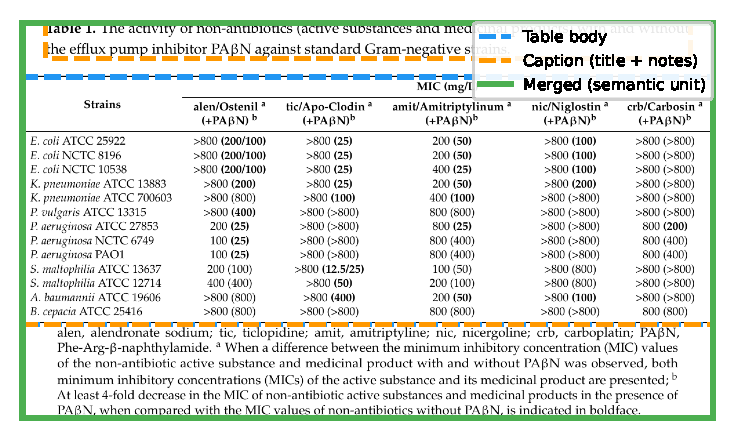
\includegraphics[width=0.55\textwidth]{figures/Fig1.pdf}
\caption{Example of a semantically complete table unit from SCI-3000. Dashed blue
indicates the table body. Dashed orange marks the caption: both the title above the
table and the descriptive notes below it. The solid green box shows the merged
semantic unit}
\label{fig:semantic_unit}
\end{figure*}

\subsection{Three Formulations}\label{sec:formulations}

Three formulations are compared, each representing a different approach to defining
the detection target. They differ in how caption content is handled: excluded,
learned jointly, or recovered through post-processing.

\textbf{Formulation~A (Table-only)} corresponds to the standard localisation target:
a bounding box enclosing only the visual table body, as used in
TATR and TableBank~\cite{li2020tablebank}.

\textbf{Formulation~B (Merged crop)} uses a single bounding box enclosing the table
body and caption(s). The detector is fine-tuned to predict this
expanded target directly.

\textbf{Formulation~C (Heuristic post-processing)} starts from a table-only detector
and applies heuristic spatial expansion, scanning for dark pixels above and below the
table body to capture caption content. This formulation is controlled by scan
distance and gap-tolerance parameters. Figure~\ref{fig:formulation_comparison}
shows the detection targets under each formulation.

\begin{figure*}[ht!]
\centering
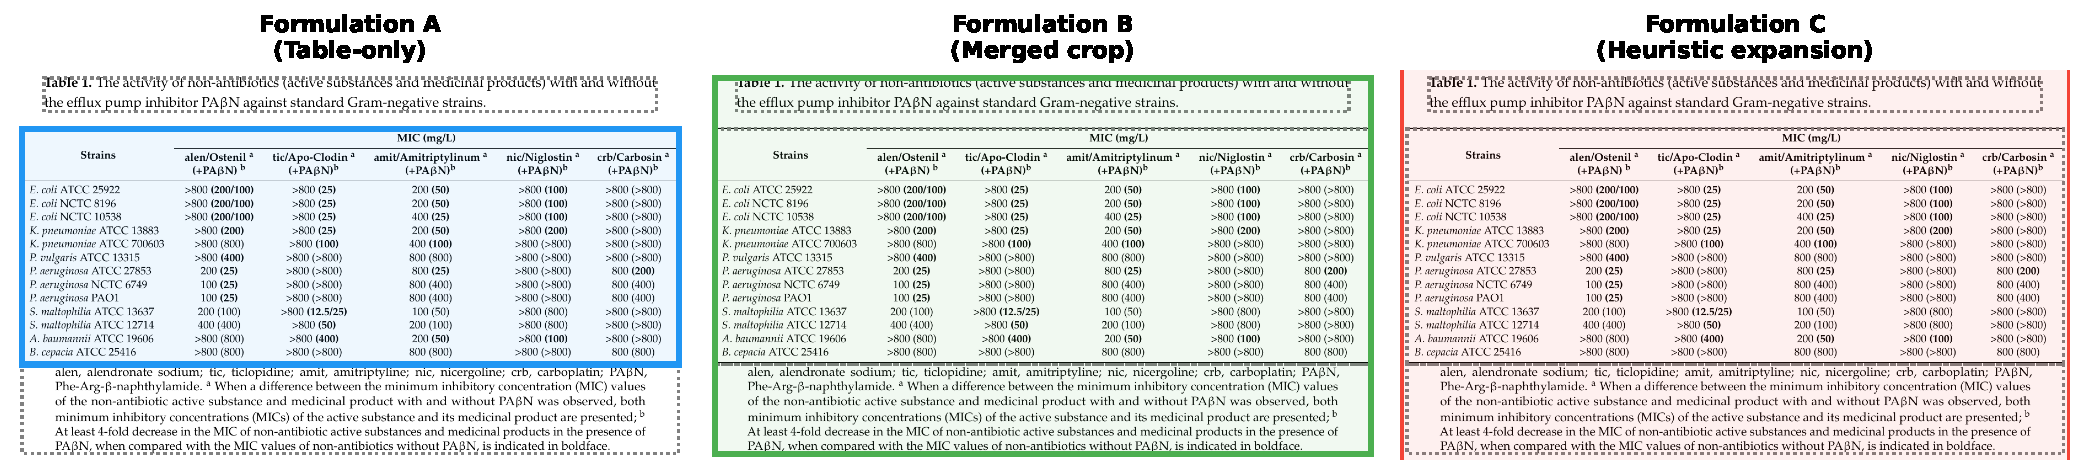
\includegraphics[width=0.95\textwidth]{figures/Fig2.pdf}
\caption{Detection targets for the same table under each formulation. Formulation~A
(left) captures only the table body. Formulation~B (centre) captures the merged
semantic unit. Formulation~C (right) applies heuristic expansion. Grey dotted lines
indicate ground truth element boundaries}
\label{fig:formulation_comparison}
\end{figure*}

\subsection{Annotation Rationale and Ambiguity Handling}\label{sec:annotation}

Because the contribution concerns the definition of the target object itself,
annotation validity is central to the study. In SCI-3000, caption association is
determined by the explicit \texttt{parent\_id} field, which links each caption
element to its parent table. When multiple caption fragments refer to the same
table, they are merged into a single bounding box. Footnotes are identified as text
elements positioned directly below the table body within a vertical distance
threshold. Continued tables spanning multiple pages are excluded because a
single-page crop cannot capture the full object. Ambiguous cases, such as captions
located between two nearby tables, are resolved by the distance-threshold rule unless
explicit linking is present. All annotations are derived deterministically from the
existing SCI-3000 schema without manual re-annotation, making the process
reproducible.

% ================================================================
\section{Methods and Datasets}\label{sec:methods}

\subsection{Detection Models}\label{sec:models}

The main experiments use the Microsoft Table Transformer
(TATR)~\cite{smock2022pubtables}, a DETR-based~\cite{carion2020detr} detector
pre-trained on PubTables-1M. TATR performs strongly on standard table-body detection
with body-only pre-training targets, making the effect of caption-aware fine-tuning
clear.

To test whether the formulation ranking depends on model architecture, a parallel
evaluation uses YOLOv26m~\cite{ultralytics2025yolo}, a single-stage anchor-free
detector with 21.8\,M parameters. YOLOv26m is fine-tuned from a COCO-pretrained
checkpoint on SCI-3000 for all three formulations using the same data split and
annotation targets (50 epochs, batch size 16, AdamW optimiser). The resulting models are evaluated with the same
completeness metrics and confidence threshold ($\tau = 0.5$) as TATR. For
Formulation~C (multi-class), only table-class detections are retained; caption-class
detections are discarded.

\subsection{Datasets}\label{sec:datasets}

\textbf{SCI-3000}~\cite{darmanovic2023sci} is a scientific document corpus available
on Zenodo containing 3\,000 pages with table, figure, and caption annotations,
including explicit \texttt{parent\_id} links between captions and parent tables. A
fixed split of 2\,003 training and 997 validation pages is used. The validation set
contains 1\,277 ground truth tables. No pages were excluded.

\textbf{PubTables-1M}~\cite{smock2022pubtables} is a large-scale table detection
dataset with table-body-only annotations. A subset of 2\,000 randomly sampled test
images is used for cross-dataset transfer evaluation.

\subsection{TATR Fine-Tuning Details}\label{sec:finetuning}

For Formulation~B, TATR is fine-tuned by replacing the table-body ground truth boxes
with merged table-plus-caption bounding boxes derived from the SCI-3000 annotations.
Training proceeds in five phases with cosine learning-rate decay from
$1 \times 10^{-5}$ to $1 \times 10^{-6}$, using AdamW with batch size 8 on a single
24GB RTX 3090 GPU. Pages are rendered at 200\,dpi and then resized to a maximum dimension
of 800\,px during training. This resolution is used to ensure consistency across all experiments while preserving sufficient detail for aligning annotation canvas coordinates with pixel positions before resizing. The detection confidence threshold is 0.7. No non-maximum
suppression is applied because DETR is inherently NMS-free. The final checkpoint
(\texttt{phase5\_resumed\_final}) achieves validation IoU\,=\,0.969 with
recall\,=\,0.998 and precision\,=\,0.984. All experiments use seed\,=\,42.

\subsection{Semantic Completeness Metrics}\label{sec:metrics}

Three complementary metrics are introduced, each capturing an aspect of semantic
adequacy that standard AP and IoU do not measure.

\textbf{Caption Inclusion Rate (CIR)} measures the fraction of ground truth caption
area captured by the predicted crop:
\begin{equation}\label{eq:cir}
\text{CIR} = \frac{|C_{\text{pred}} \cap C_{\text{gt}}|}{|C_{\text{gt}}|},
\end{equation}
where $C_{\text{pred}}$ is the caption area within the predicted crop and
$C_{\text{gt}}$ is the total ground truth caption area.

\textbf{Semantic Coverage Score (SCS)} measures coverage of all semantic components
(table body, caption, and footnotes), weighted by area.

\textbf{Complete Unit Capture Rate (CUCR)} is a binary per-table score equal to 1 if
both the table body and all linked captions have IoU $\geq 0.5$ with the predicted
crop. It reflects whether the full interpretable unit has been captured.

The \textbf{over-crop ratio} is also reported: the fraction of predicted crop area
that lies outside the ground truth merged target, penalising expansion that includes
irrelevant content. Figure~\ref{fig:metric_schematic} shows how a standard
table-body detection can differ from a merged crop, illustrating why standard AP and
completeness metrics can diverge.

\begin{figure*}[ht!]
\centering
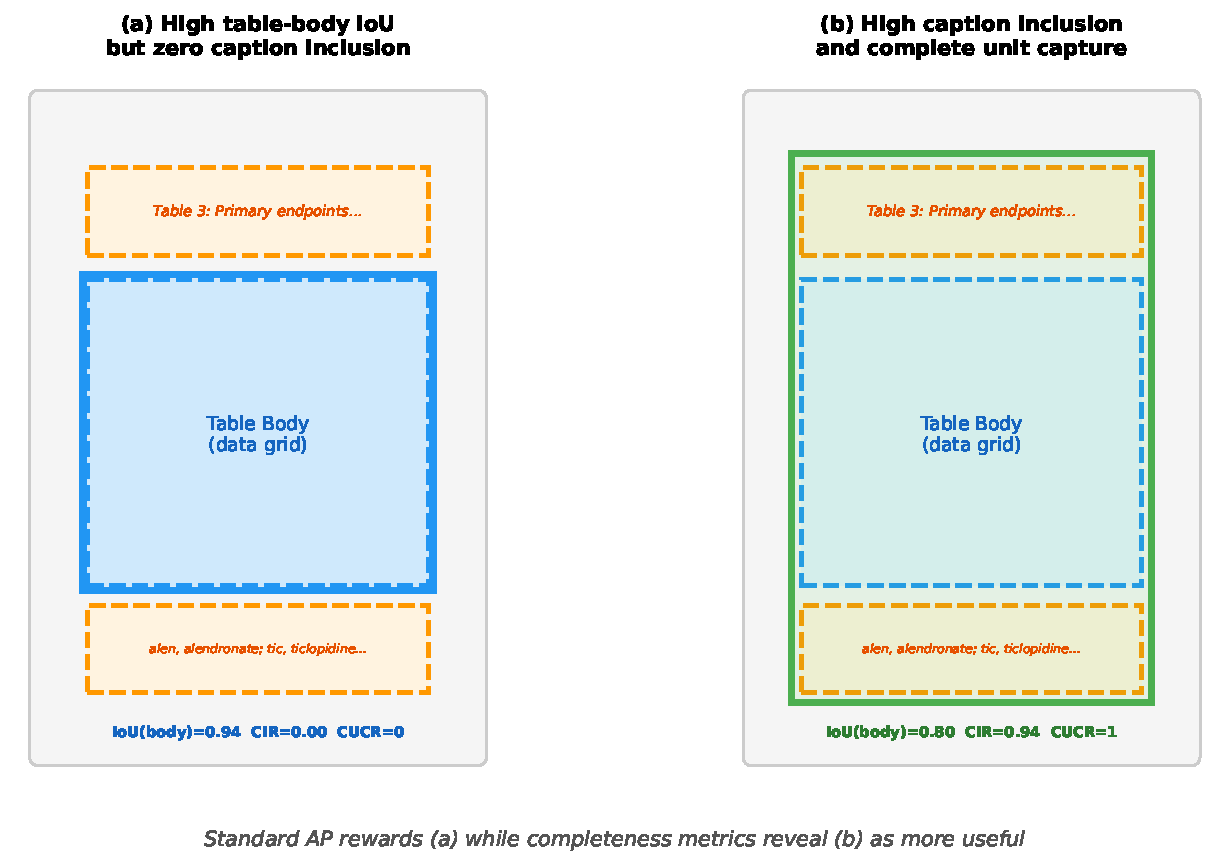
\includegraphics[width=0.75\textwidth]{figures/Fig3.pdf}
\caption{Why standard AP and completeness metrics can disagree. (a) A table-body
detection achieves high body IoU but zero caption inclusion. (b) A merged crop has
slightly lower body IoU but captures the caption and the complete semantic unit. Line
styles: dashed blue = table body, dashed orange = caption, solid box = detection
output}
\label{fig:metric_schematic}
\end{figure*}

% ================================================================
\section{Experiments and Results}\label{sec:experiments}

\subsection{TATR Formulation Comparison}\label{sec:tatr_comparison}

Table~\ref{tab:tatr_results} presents the main formulation comparison on the SCI-3000
validation set (1\,277 tables, seed\,=\,42). Formulation~B achieves high merged-target
detection (AP@50\,=\,0.989, mAP\,=\,0.964), strong completeness
(CIR\,=\,94.2\%, CUCR\,=\,78.1\%), and controlled over-crop (11.1\%).
Formulation~A achieves the highest table-body AP (0.944) but captures only 0.4\% of
caption area. Formulation~C reaches similar caption coverage (CIR\,=\,93.9\%) but
with substantially higher over-crop (41.7\%) and lower detection quality against the
merged target.

\begin{table}[ht!]
\caption{TATR formulation comparison on the SCI-3000 validation set
(1\,277 tables). Best values are shown in \textbf{bold}.}
\label{tab:tatr_results}
\footnotesize\setlength{\tabcolsep}{3pt}
\begin{tabular}{@{}lccc@{}}
\toprule
\textbf{Metric} & \textbf{A: Table-only} & \textbf{B: Merged (FT)} & \textbf{C: Heuristic} \\
\midrule
AP@50 (merged) & 0.770 & \textbf{0.989} & 0.412 \\
AP@75 (merged) & 0.223 & \textbf{0.977} & 0.122 \\
mAP (merged) & 0.324 & \textbf{0.964} & 0.172 \\
\midrule
CIR & 0.4\% & \textbf{94.2\%} & 93.9\% \\
SCS & 42.0\% & \textbf{96.5\%} & 95.5\% \\
CUCR & 0.0\% & \textbf{78.1\%} & 24.1\% \\
Over-crop & \textbf{0.4\%} & 11.1\% & 41.7\% \\
\midrule
Table-body IoU & \textbf{0.834} & 0.799 & 0.522 \\
AP@50 (table-only) & \textbf{0.944} & 0.917 & 0.308 \\
\bottomrule
\end{tabular}
\end{table}

\subsection{Cross-Architecture Consistency (YOLOv26m)}\label{sec:yolo_results}

The same formulations are evaluated with YOLOv26m, a single-stage detector
independently fine-tuned on SCI-3000 (see Section~\ref{sec:models}).
Table~\ref{tab:yolo_results} shows that the ranking holds across both detector
families: Formulation~B achieves the highest caption inclusion and complete-unit
capture, while Formulations~A and~C capture almost no caption content.

\begin{table}[ht!]
\caption{YOLOv26m completeness evaluation on SCI-3000
(same split and metrics as Table~\ref{tab:tatr_results}). The formulation
ranking is consistent with TATR.}
\label{tab:yolo_results}
\footnotesize\setlength{\tabcolsep}{3pt}
\begin{tabular}{@{}lccc@{}}
\toprule
\textbf{Metric} & \textbf{A: Table-only} & \textbf{B: Merged} & \textbf{C: Multi-class} \\
\midrule
mAP@50-95 (train) & 0.978 & \textbf{0.984} & 0.913 \\
AP@50 (table-only) & \textbf{0.968} & 0.909 & 0.938 \\
\midrule
CIR & 0.8\% & \textbf{97.4\%} & 0.6\% \\
SCS & 49.4\% & \textbf{98.2\%} & 49.5\% \\
CUCR & 0.6\% & \textbf{80.3\%} & 0.3\% \\
Over-crop & \textbf{1.1\%} & 10.7\% & 1.3\% \\
\midrule
Table-body IoU & \textbf{0.969} & 0.802 & 0.971 \\
\bottomrule
\end{tabular}
\end{table}

Two patterns are consistent across architectures. Formulation~B delivers
near-complete caption capture (CIR\,=\,97.4\%, CUCR\,=\,80.3\%) with controlled
over-crop (10.7\%), closely matching the TATR pattern. Formulations~A and~C both
achieve high table-body localisation (IoU $> 0.96$) but near-zero caption inclusion,
confirming that body-only detection targets exclude caption content regardless of
architecture.

\subsection{Statistical Validation}\label{sec:bootstrap}

Bootstrap 95\% confidence intervals are computed using 10\,000 resamples of per-table
completeness scores~\cite{efron1993bootstrap} to assess sampling variability.
Table~\ref{tab:bootstrap} shows clear separation between formulations on all
completeness metrics, particularly CUCR and over-crop ratio.

\begin{table}[ht!]
\caption{Bootstrap 95\% CIs for completeness metrics
(10\,000 resamples). Point estimates with bounds in brackets.}
\label{tab:bootstrap}
\footnotesize\setlength{\tabcolsep}{3pt}
\begin{tabular}{@{}lccc@{}}
\toprule
\textbf{Metric} & \textbf{A} & \textbf{B} & \textbf{C} \\
\midrule
CIR & .004 [.001, .007] & \textbf{.942} [.935, .947] & .940 [.931, .948] \\
SCS & .420 [.417, .424] & \textbf{.965} [.961, .968] & .955 [.950, .961] \\
CUCR & .000 [.000, .000] & \textbf{.781} [.758, .803] & .241 [.218, .265] \\
Over-crop & \textbf{.004} [.003, .005] & .111 [.106, .116] & .417 [.404, .431] \\
Table IoU & \textbf{.834} [.827, .840] & .799 [.792, .807] & .522 [.510, .535] \\
\bottomrule
\end{tabular}
\end{table}

\subsection{Heuristic Sensitivity Analysis}\label{sec:sensitivity}

Table~\ref{tab:sweep} reports the sensitivity of Formulation~C to its expansion
parameters. Figure~\ref{fig:heuristic_failures} shows examples of heuristic expansion
failures.

\begin{figure*}[ht!]
\centering
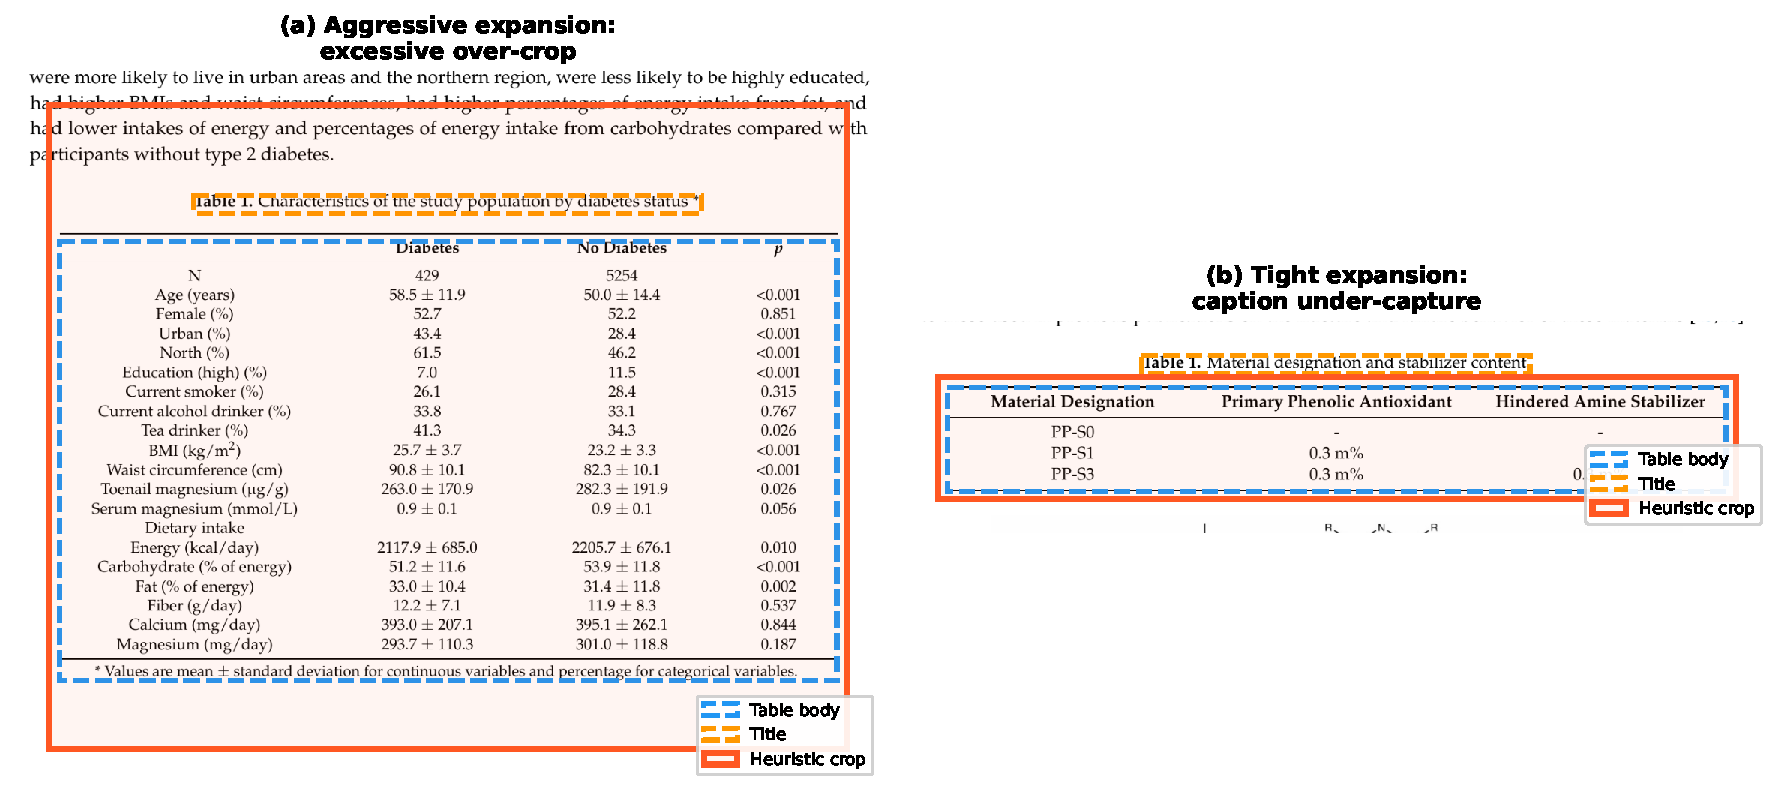
\includegraphics[width=0.95\textwidth]{figures/Fig4.pdf}
\caption{Examples of heuristic expansion failure. (a) Aggressive expansion captures the
caption but also includes surrounding body text, producing high over-crop. (b) Tight
expansion misses the caption entirely and yields a semantically incomplete crop. Line
styles distinguish elements: dashed blue = table body, dashed orange = caption, solid
red = heuristic crop}
\label{fig:heuristic_failures}
\end{figure*}

\begin{table}[ht!]
\caption{Heuristic sensitivity sweep for Formulation~C (1\,265 tables). CUCR peaks at
the conservative setting but remains below Formulation~B (0.781).}
\label{tab:sweep}
\footnotesize\setlength{\tabcolsep}{3pt}
\begin{tabular}{@{}lccccc@{}}
\toprule
& \textbf{Tight} & \textbf{Consv.} & \textbf{Default} & \textbf{Aggr.} & \textbf{Max.} \\
\midrule
pad\_top (px) & 80 & 150 & \textbf{250} & 350 & 500 \\
pad\_bot (px) & 100 & 200 & \textbf{400} & 500 & 700 \\
gap\_tol (px) & 30 & 40 & \textbf{60} & 80 & 100 \\
\midrule
CIR & 0.611 & 0.919 & 0.940 & 0.950 & 0.957 \\
CUCR & 0.478 & \textbf{0.627} & 0.241 & 0.103 & 0.064 \\
Over-crop & \textbf{0.095} & 0.164 & 0.417 & 0.543 & 0.625 \\
Table IoU & \textbf{0.817} & 0.738 & 0.522 & 0.413 & 0.342 \\
\bottomrule
\end{tabular}
\end{table}

CUCR peaks at the \textit{conservative} setting (0.627) and falls as
expansion widens and over-crop increases. The best heuristic setting remains below
the learned merged model (CUCR\,=\,0.781), indicating that no single heuristic
configuration matches the coverage and precision balance of Formulation~B.

\subsection{Metric Robustness}\label{sec:robustness}

Table~\ref{tab:cucr_sensitivity} reports CUCR at five IoU thresholds to verify that
the conclusions are not sensitive to threshold choice. Formulation~B leads at every
threshold, ranging from 0.976 at 0.4 to 0.578 at 0.8. Formulation~C peaks at 0.630
under lenient matching but falls to 0.137 at the strictest threshold.
Formulation~A remains near zero throughout. SCS is similarly robust to alternative
component-weighting schemes: equal weighting (B\,=\,0.965), body-heavy 2:1:1
(B\,=\,0.972), and caption-heavy 1:2:1 (B\,=\,0.957) all preserve the same ranking.

\begin{table}[ht!]
\caption{CUCR at varying IoU thresholds. Formulation~B leads at all thresholds.}
\label{tab:cucr_sensitivity}
\footnotesize\setlength{\tabcolsep}{4pt}
\begin{tabular}{@{}lccc@{}}
\toprule
\textbf{IoU} & \textbf{A} & \textbf{B} & \textbf{C} \\
\midrule
0.4 & 0.005 & \textbf{0.976} & 0.630 \\
0.5 & 0.002 & \textbf{0.940} & 0.483 \\
0.6 & 0.001 & \textbf{0.879} & 0.355 \\
0.7 & 0.000 & \textbf{0.781} & 0.241 \\
0.8 & 0.000 & \textbf{0.578} & 0.137 \\
\bottomrule
\end{tabular}
\end{table}

Figure~\ref{fig:scatter} shows the per-table coverage and precision trade-off. Each
point represents one table; large markers indicate formulation means.
Formulation~A clusters at low over-crop but low SCS (mean: 0.004, 0.420).
Formulation~C achieves high SCS at the cost of high over-crop (mean: 0.417, 0.955).
Formulation~B sits near the best frontier, combining high SCS with controlled
over-crop (mean: 0.111, 0.965).

\begin{figure}[ht!]
\centering
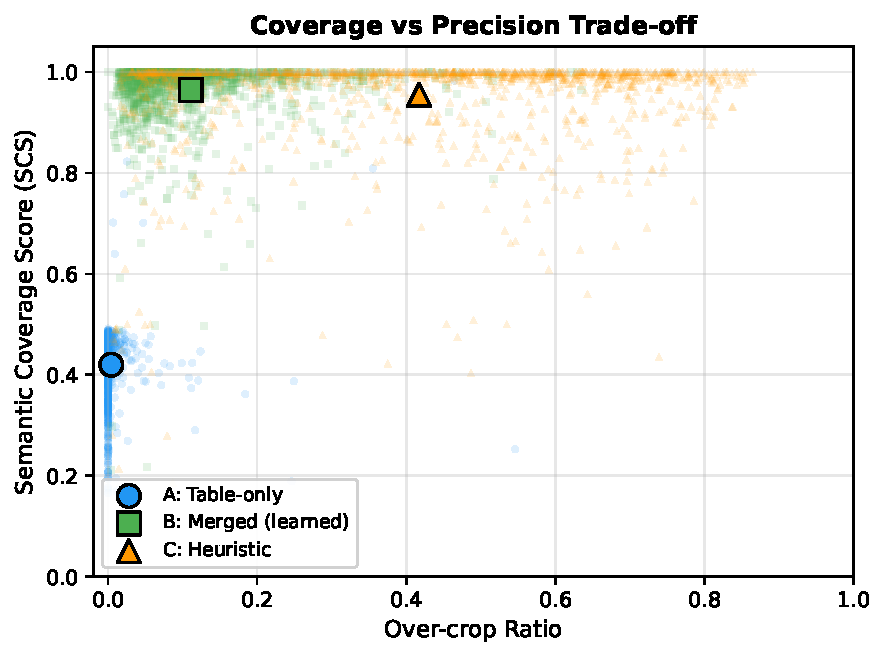
\includegraphics[width=0.85\columnwidth]{figures/Fig5.pdf}
\caption{Per-table over-crop ratio versus Semantic Coverage Score. Each point is one
table; large markers show formulation means. Formulation~B achieves the best
balance of coverage and precision}
\label{fig:scatter}
\end{figure}

\subsection{Cross-Dataset Transfer}\label{sec:transfer}

The fine-tuned model is evaluated on PubTables-1M test images to assess whether
caption-aware fine-tuning harms general table localisation.
Table~\ref{tab:transfer} shows that Formulation~B incurs only a 2.0\% AP@50
reduction relative to the pre-trained baseline. Larger reductions at AP@75 and mean
IoU are expected because the fine-tuned model predicts expanded boxes, whereas
PubTables-1M ground truth covers only the table body.

\begin{table}[ht!]
\caption{Cross-dataset transfer on PubTables-1M (2\,000 images). AP@50 decreases by
only 2.0\%.}
\label{tab:transfer}
\footnotesize\setlength{\tabcolsep}{3pt}
\begin{tabular}{@{}lccc@{}}
\toprule
\textbf{Metric} & \textbf{Pre-trained} & \textbf{Fine-tuned (B)} & $\Delta$ \\
\midrule
AP@50 & 0.909 & 0.889 & $-$0.020 \\
AP@75 & 0.909 & 0.480 & $-$0.429 \\
Recall@50 & 1.000 & 0.943 & $-$0.057 \\
Mean IoU & 0.978 & 0.755 & $-$0.223 \\
\bottomrule
\end{tabular}
\end{table}

% ================================================================
\section{Downstream Extraction Validation}\label{sec:downstream}

A downstream extraction experiment tests whether the observed completeness
differences have practical consequences. A multimodal LLM (GPT-5.2, accessed via
OpenRouter API; temperature\,=\,0; \texttt{max\_tokens}\,=\,2\,048;
structured JSON output) extracts information from crop images produced by each
formulation. One hundred tables are sampled from the SCI-3000 validation set,
selecting cases with verified caption associations. Crop images are encoded as
base64 PNG and resized to a maximum dimension of 1\,568\,px. Title extraction is
scored as successful if the model returns a non-null title string of length greater
than five characters. Full scoring rules are documented in
Appendix~\ref{app:prompts}. This experiment provides application-oriented
validation rather than a full benchmark of extraction models.

\subsection{Tier~1: Title and Study Arm Extraction}\label{sec:tier1}

Table~\ref{tab:downstream_t1} shows that Formulation~A yields only a 2\% title
extraction rate. Both Formulations~B (94\%) and~C (95\%) include the caption
frequently enough to support reliable title extraction. Study-arm identification is
similar across formulations because this information is typically encoded within the
table body. Omitting caption content sharply constrains caption-dependent extraction.

\begin{table}[ht!]
\caption{Tier~1 downstream extraction on 100 tables. Title extraction is near-zero for
table-only crops.}
\label{tab:downstream_t1}
\footnotesize\setlength{\tabcolsep}{3pt}
\begin{tabular}{@{}lccc@{}}
\toprule
\textbf{Metric} & \textbf{A} & \textbf{B} & \textbf{C} \\
\midrule
Title extraction rate & 2.0\% & \textbf{94.0\%} & 95.0\% \\
Caption visible & 2.0\% & 94.0\% & 95.0\% \\
Mean study arms found & 3.4 & 3.4 & 3.5 \\
\bottomrule
\end{tabular}
\end{table}

\subsection{Tier~2: Full Field Extraction}\label{sec:tier2}

Table~\ref{tab:downstream_t2} reports full field extraction. Title extraction remains
the clearest separator: 4\% for Formulation~A, 88\% for~B, and 79\% for~C. The gap
between B and C in this more demanding setting suggests that learned merged detection
provides more reliable caption inclusion than heuristic expansion. Table-body
extraction (columns, rows, and numeric values recovered) is comparable across
formulations, consistent with all three capturing the table body.

\begin{table}[ht!]
\caption{Tier~2 downstream extraction on 100 tables. Formulation~B outperforms
Formulation~C on title extraction (88\% versus 79\%).}
\label{tab:downstream_t2}
\footnotesize\setlength{\tabcolsep}{3pt}
\begin{tabular}{@{}lccc@{}}
\toprule
\textbf{Metric} & \textbf{A} & \textbf{B} & \textbf{C} \\
\midrule
Title extraction rate & 4.0\% & \textbf{88.0\%} & 79.0\% \\
Mean columns & 4.3 & 4.3 & 4.2 \\
Mean rows & 8.6 & 7.8 & 7.9 \\
Mean values extracted & \textbf{32.4} & 29.4 & 29.1 \\
\bottomrule
\end{tabular}
\end{table}

% ================================================================
\section{Discussion}\label{sec:discussion}

\subsection{Implications for Benchmark Design}\label{sec:benchmarks}

The results suggest that benchmark definitions for table detection should align with
the intended downstream unit of analysis. When the task is document understanding or
information extraction, evaluation against the table body alone can favour detectors
that are geometrically accurate yet semantically incomplete. Formulation~A achieves
the highest table-body AP (0.944) but captures almost no caption content and yields
zero complete unit capture. This divergence shows that AP against body-only targets
is insufficient when the goal is an interpretable table unit.

\subsection{Implications for Document Understanding Pipelines}\label{sec:pipelines}

Formulation~B is the only method that combines high semantic completeness with
moderate over-crop. Its CUCR (78.1\% versus 24.1\% for Formulation~C) and over-crop
ratio (11.1\% versus 41.7\%) confirm this balance. The downstream validation
supports this finding: Formulation~B achieves the highest title extraction rate
across both tiers, while Formulation~C is less reliable in the more demanding
Tier~2 setting.

The heuristic sensitivity analysis supports the same conclusion. No single
parameter configuration for Formulation~C achieves both high caption coverage and
low over-crop. As expansion widens, caption inclusion improves, but complete-unit
capture deteriorates because the crop increasingly includes irrelevant content.
This trade-off appears inherent to spatial heuristics that do not model document
semantics.

\subsection{Limitations}\label{sec:limitations}

This study has several limitations. First, it is limited to English-language
scientific documents and single-page table units in SCI-3000. The annotation rules
may require adaptation for other genres, including financial reports, legal
documents, and scanned historical records~\cite{granell2023historical,andres2025pares}.
Second, the downstream validation uses a single multimodal extraction system and is
better interpreted as a practical case study than a comprehensive comparison of
extraction models. Third, the evaluation focuses on captions as the contextual
element; footnote coverage is addressed in the definition and metrics but is not
extensively validated empirically, because SCI-3000 does not annotate footnotes as a
separate class. Fourth, the cross-dataset transfer evaluation is constrained by
PubTables-1M's table-body-only annotations, which systematically penalise models
trained to predict expanded bounding boxes. Finally, while the formulation ranking
is consistent across two detector families (TATR and YOLOv26m), extending the
comparison to additional architectures and domains remains a direction for future
work.

\subsection{Generalisation and Future Work}\label{sec:future}

The cross-dataset transfer results provide initial evidence that caption-aware
fine-tuning does not substantially harm general table localisation, with only a
2.0\% AP@50 reduction on PubTables-1M. Broader cross-domain evaluation remains
necessary, including on financial, historical, and engineering
documents~\cite{zhang2022yolotable,song2024robust}. Future work could explore
learned table-caption linking as an alternative to heuristic association in
Formulation~C, and benchmark extensions that annotate captions explicitly so that
semantic completeness can be evaluated in a standardised way.

% ================================================================
\section{Conclusion}\label{sec:conclusion}

This paper formalises caption-aware table-region extraction as a document analysis
task, compares three target formulations across two detector architectures,
introduces completeness metrics, and shows their practical consequences. The learned
merged formulation achieves high detection performance (AP@50\,=\,0.989), strong
caption inclusion (94.2\%), and controlled over-crop (11.1\%). Standard AP metrics
do not capture this distinction: the table-only formulation scores highest on
table-body AP while omitting almost all caption content. Heuristic expansion
improves caption coverage but remains sensitive to parameter choice and does not
match the balance of the learned merged model.

The choice of detection target is itself a design decision with measurable
consequences. When the detection target does not match the unit that downstream
systems need, strong localisation performance can coexist with limited practical
usefulness. For scientific documents, caption-aware table extraction provides a more
appropriate evaluation unit and a stronger foundation for document understanding
pipelines.

% Back matter ====================================================
\backmatter

\section*{Declarations}

\begin{description}
\item[Funding] No funding was received for conducting this study.
\item[Competing interests] The author has no competing interests to declare.
\item[Ethics approval] Not applicable.
\item[Consent to participate] Not applicable.
\item[Consent for publication] Not applicable.
\item[Data availability] The SCI-3000 dataset is available from Zenodo at \url{https://doi.org/10.5281/zenodo.8357124}. PubTables-1M is available from~\cite{smock2022pubtables}.
\item[Code availability] Repository link will be provided once paper is accepted.

\item[Use of AI tools] A multimodal LLM-based system (GPT-5.2) was used only in the downstream extraction experiment described in Section~\ref{sec:downstream}. No AI tools were used in the writing of the manuscript or in the interpretation of results.
\end{description}

\begin{thebibliography}{00}

\bibitem{ultralytics2025yolo}
Jocher, G., Qiu, J., Chaurasia, A.:
Ultralytics YOLO26 (2026).
\url{https://github.com/ultralytics/ultralytics}

\bibitem{smock2022pubtables}
Smock, B., Pesala, R., Abraham, R.:
PubTables-1M: Towards comprehensive table extraction from unstructured documents.
In: IEEE/CVF Conference on Computer Vision and Pattern Recognition (CVPR),
pp.~4624--4632 (2022).
\url{https://doi.org/10.1109/CVPR52688.2022.00459}

\bibitem{hashmi2021survey}
Hashmi, K.A., Liwicki, M., Stricker, D., Afzal, M.A., Afzal, M.Z.:
Current status and performance analysis of table recognition in document
images with deep neural networks.
IEEE Access \textbf{9}, 87663--87685 (2021).
\url{https://doi.org/10.1109/ACCESS.2021.3087865}

\bibitem{marshall2019toward}
Marshall, I.J., Wallace, B.C.:
Toward systematic review automation: A practical guide to using machine learning
tools in research synthesis.
Syst.\ Rev.\ \textbf{8}(1), 163 (2019).
\url{https://doi.org/10.1186/s13643-019-1074-9}

\bibitem{carion2020detr}
Carion, N., Massa, F., Synnaeve, G., Usunier, N., Kirillov, A., Zagoruyko, S.:
End-to-end object detection with transformers.
In: European Conference on Computer Vision (ECCV), pp.~213--229. Springer (2020)

\bibitem{ren2017faster}
Ren, S., He, K., Girshick, R., Sun, J.:
Faster R-CNN: Towards real-time object detection with region proposal networks.
IEEE Trans.\ Pattern Anal.\ Mach.\ Intell.\ \textbf{39}(6), 1137--1149 (2017).
\url{https://doi.org/10.1109/TPAMI.2016.2577031}

\bibitem{redmon2016yolo}
Redmon, J., Divvala, S., Girshick, R., Farhadi, A.:
You only look once: Unified, real-time object detection.
In: IEEE/CVF Conference on Computer Vision and Pattern Recognition (CVPR),
pp.~779--788 (2016)

\bibitem{zhang2022yolotable}
Zhang, D., Mao, R., Guo, R., Jiang, Y., Zhu, J.:
YOLO-table: Disclosure document table detection with involution.
Int.\ J.\ Doc.\ Anal.\ Recognit.\ \textbf{26}, 1--14 (2023).
\url{https://doi.org/10.1007/s10032-022-00400-z}

\bibitem{hashmi2021castabdetectors}
Hashmi, K.A., Pagani, A., Liwicki, M., Stricker, D., Afzal, M.Z.:
CasTabDetectoRS: Cascade network for table detection in document images with
recursive feature pyramid and switchable atrous convolution.
J.\ Imaging \textbf{7}(10), 214 (2021).
\url{https://doi.org/10.3390/jimaging7100214}

\bibitem{ehsan2024semisupervised}
Ehsan, T., Shehzadi, T., Stricker, D., Afzal, M.Z.:
End-to-end semi-supervised approach with modulated object queries for table
detection in documents.
Int.\ J.\ Doc.\ Anal.\ Recognit.\ \textbf{27}, 207--226 (2024).
\url{https://doi.org/10.1007/s10032-024-00471-0}

\bibitem{song2024robust}
Song, L., Huang, X., Zhuang, S., Shen, A., Xu, P.:
Robust table structure recognition network based on local and global perspectives.
IEEE Access \textbf{12}, 138279--138291 (2024).
\url{https://doi.org/10.1109/ACCESS.2024.3458946}

\bibitem{li2020tablebank}
Li, M., Cui, L., Huang, S., Wei, F., Zhou, M., Li, Z.:
TableBank: Table benchmark for image-based table detection and recognition.
In: International Conference on Language Resources and Evaluation (LREC),
pp.~1918--1925 (2020)

\bibitem{hong2025vertexnet}
Hong, T., Yang, Y.:
VertexNet: A table structure recognition model based on key points for complex scenes.
Int.\ J.\ Doc.\ Anal.\ Recognit.\ \textbf{28}(4), 30 (2025).
\url{https://doi.org/10.1007/s10032-025-00516-y}

\bibitem{wang2023scene}
Wang, H., Xue, Y., Zhang, J., Jin, L.:
Scene table structure recognition with segmentation collaboration and alignment.
Pattern Recognit.\ Lett.\ \textbf{165}, 68--75 (2023).
\url{https://doi.org/10.1016/j.patrec.2022.12.014}

\bibitem{kayal2022tables}
Kayal, P., Anand, M., Desai, H., Singh, M.:
Tables to LaTeX: Structure and content extraction from scientific tables.
Int.\ J.\ Doc.\ Anal.\ Recognit.\ \textbf{25}, 307--323 (2022).
\url{https://doi.org/10.1007/s10032-022-00420-9}

\bibitem{li2020docbank}
Li, M., Xu, Y., Cui, L., Huang, S., Wei, F., Li, Z., Zhou, M.:
DocBank: A benchmark dataset for document layout analysis.
In: International Conference on Computational Linguistics (COLING),
pp.~949--960 (2020)

\bibitem{xu2020layoutlm}
Xu, Y., Li, M., Cui, L., Huang, S., Wei, F., Zhou, M.:
LayoutLM: Pre-training of text and layout for document image understanding.
In: ACM SIGKDD International Conference on Knowledge Discovery and Data Mining
(KDD), pp.~1192--1200 (2020)

\bibitem{huang2022layoutlmv3}
Huang, Y., Lv, T., Cui, L., Lu, Y., Wei, F.:
LayoutLMv3: Pre-training for document AI with unified text and image masking.
In: ACM International Conference on Multimedia (MM), pp.~4083--4091 (2022).
\url{https://doi.org/10.1145/3503161.3548112}

\bibitem{prasad2020cascadetabnet}
Prasad, D., Gadpal, A., Kapadni, K., Visave, M., Sultanpure, K.:
CascadeTabNet: An approach for end to end table detection and structure recognition
from image-based documents.
In: IEEE/CVF CVPR Workshops (CVPRW) (2020)

\bibitem{lopez2009grobid}
Lopez, P.:
GROBID: Combining automatic bibliographic data recognition and term extraction for
scholarship publications.
In: European Conference on Digital Libraries (ECDL), pp.~473--474 (2009)

\bibitem{lo2020s2orc}
Lo, K., Wang, L.L., Neumann, M., Kinney, R., Weld, D.S.:
S2ORC: The Semantic Scholar Open Research Corpus.
In: Annual Meeting of the Association for Computational Linguistics (ACL),
pp.~4969--4983 (2020)

\bibitem{milosevic2019biomedical}
Milosevic, N., Gregson, C., Hernandez, R., Nenadic, G.:
A framework for information extraction from tables in biomedical literature.
Int.\ J.\ Doc.\ Anal.\ Recognit.\ \textbf{22}, 55--78 (2019).
\url{https://doi.org/10.1007/s10032-019-00317-0}

\bibitem{lin2014coco}
Lin, T.-Y., Maire, M., Belongie, S., Hays, J., Perona, P., Ramanan, D.,
Doll\'{a}r, P., Zitnick, C.L.:
Microsoft COCO: Common objects in context.
In: European Conference on Computer Vision (ECCV), pp.~740--755. Springer (2014)

\bibitem{xiao2023improved}
Xiao, B., Simsek, M., Kantarci, B., Alkheir, A.A.:
Table detection for visually rich document images.
Knowl.-Based Syst.\ \textbf{282}, 111080 (2023).
\url{https://doi.org/10.1016/j.knosys.2023.111080}

\bibitem{xiao2025revisiting}
Xiao, B., Simsek, M., Kantarci, B., Alkheir, A.A.:
Revisiting table detection datasets for visually rich documents.
Int.\ J.\ Doc.\ Anal.\ Recognit.\ (2025).
\url{https://doi.org/10.1007/s10032-025-00527-9}

\bibitem{efron1993bootstrap}
Efron, B., Tibshirani, R.J.:
An Introduction to the Bootstrap.
Chapman \& Hall/CRC (1993).
\url{https://doi.org/10.1007/978-1-4899-4541-9}

\bibitem{granell2023historical}
Granell, E., Romero, V., Prieto, J.R., Andr\'{e}s, J., Quir\'{o}s, L.,
S\'{a}nchez, J.A., Vidal, E.:
Processing a large collection of historical tabular images.
Pattern Recognit.\ Lett.\ \textbf{170}, 98--105 (2023).
\url{https://doi.org/10.1016/j.patrec.2023.04.007}

\bibitem{andres2025pares}
Andr\'{e}s, J., Wall, C., Tarride, S., Coustaty, M., Toselli, A.H., Vidal, E.:
The PARES Database: Information extraction over historical parish records.
Int.\ J.\ Doc.\ Anal.\ Recognit.\ (2025).
\url{https://doi.org/10.1007/s10032-025-00531-z}

\bibitem{darmanovic2023sci}
Darmanovi\'{c}, F., Hanbury, A., Zlabinger, M.:
SCI-3000: A dataset for extracting figures, tables, and captions from scientific PDFs.
Zenodo (2023).
\url{https://doi.org/10.5281/zenodo.8357124}

\end{thebibliography}

% ================================================================
% APPENDICES
% ================================================================
\begin{appendices}

\section{Annotation Derivation}\label{app:annotations}

Training and evaluation targets for each formulation are derived deterministically
from the public SCI-3000 annotations, without manual re-annotation.

\subsection*{Source Annotations}

SCI-3000 annotations follow the W3C Web Annotation format, with one JSON file per
page. Each annotation specifies a class (\texttt{Table}, \texttt{Figure}, or
\texttt{Caption}) and a bounding box in canvas coordinates
(\texttt{xywh=pixel:x,y,w,h}). Captions are linked to their parent table or figure
via a \texttt{parent\_id} field.

\subsection*{Coordinate Conversion}

SCI-3000 annotations use canvas coordinates, which must be converted to pixel
coordinates in the rendered image. Pages are rendered at 200\,dpi using
\texttt{pdf2image}. The conversion applies:
\begin{equation*}
\text{scale}_x = \frac{W_{\text{image}}}{W_{\text{canvas}}}, \quad
\text{scale}_y = \frac{H_{\text{image}}}{H_{\text{canvas}}}.
\end{equation*}
All bounding boxes are scaled by these factors before use in training or evaluation.

\subsection*{Target Derivation by Formulation}

\textbf{Formulation~A} (table-only): Each \texttt{Table} annotation maps directly to
one bounding box. Captions are ignored. No merging is applied.

\textbf{Formulation~B} (merged): For each \texttt{Table}, all \texttt{Caption}
annotations whose \texttt{parent\_id} matches the table's \texttt{id} are collected.
The merged box is computed as:
\begin{align*}
x_0 &= \min(x_0^{\text{table}}, x_0^{\text{cap}_1}, \ldots), \\
y_0 &= \min(y_0^{\text{table}}, y_0^{\text{cap}_1}, \ldots), \\
x_1 &= \max(x_1^{\text{table}}, x_1^{\text{cap}_1}, \ldots), \\
y_1 &= \max(y_1^{\text{table}}, y_1^{\text{cap}_1}, \ldots).
\end{align*}
Tables with no linked caption use the table-only box (no expansion).
Approximately 15\% of tables in SCI-3000 have no linked caption, 3\% have multiple
caption fragments, and 5\% of captions lack a \texttt{parent\_id} and are excluded.

\textbf{Formulation~C} (heuristic): Tables and captions are separate detection targets
(class~0: table, class~1: caption). Only captions with a valid \texttt{parent\_id}
pointing to a table are included; unlinked captions are excluded to reduce noise.

\subsection*{Filtering and Exclusions}

Three filters are applied: (1)~pages without any table annotations are excluded;
(2)~duplicate annotations with IoU\,$>$\,0.9 are de-duplicated; (3)~boxes with area
below 100 canvas-coordinate pixels are excluded as probable annotation errors.

\subsection*{PubTables-1M Conversion}

For cross-dataset transfer evaluation, PubTables-1M annotations in PASCAL VOC XML
format are converted to the same evaluation schema. The classes \texttt{table} and
\texttt{table rotated} are mapped to a single table class. A subset of 2\,000 randomly
sampled test images is used.

% ----------------------------------------------------------------

\section{Training Details}\label{app:training}

\subsection*{Architecture Adaptation}

The Microsoft Table Transformer (TATR) is pre-trained on PubTables-1M with two
output classes (\texttt{table}, \texttt{table\_rotated}). For Formulation~B, the
classification head is reinitialised with a single output class
(\texttt{table\_with\_caption}) using Xavier uniform initialisation with zero bias.
The bounding-box regression head is retained from pre-training.

\subsection*{Training Procedure}

Fine-tuning proceeds in five phases with progressively refined ground truth
data:\vspace{0.3em}

\noindent\textbf{Phases~1--3} use the initial annotation derivation. Eight training
rounds of five epochs each are run with AdamW (batch size~8), using a differential
learning-rate scheme: $10\times$ base LR for the classification head, $1\times$ for
the box predictor, and $0.1\times$ for the backbone. After each round, precision,
recall, mean IoU, and false-positive rate on negative pages are evaluated. Rounds
that degrade any metric by more than 2\,pp are discarded and the model is rolled
back. The learning rate is increased by $3\times$ when two consecutive rounds show
no improvement.\vspace{0.3em}

\noindent\textbf{Phase~4} retrains from the pre-trained weights using tighter ground
truth annotations (reduced gap tolerance from 25 to 15\,px, reduced bottom padding
from 150 to 100\,px). Six rounds improve IoU from 0.727 to 0.883.\vspace{0.3em}

\noindent\textbf{Phase~5} retrains on the final annotation set with the cleanest
ground truth. The final checkpoint achieves all convergence targets in a single
resumed round, with IoU improving from 0.847 to 0.969.

\begin{table}[ht!]
\caption{Convergence targets and final values for TATR fine-tuning.}
\label{tab:training_targets}
\footnotesize\setlength{\tabcolsep}{3pt}
\begin{tabular}{@{}lcc@{}}
\toprule
\textbf{Metric} & \textbf{Target} & \textbf{Final} \\
\midrule
Recall & $\geq$ 0.95 & 0.998 \\
Precision & $\geq$ 0.97 & 0.984 \\
Mean IoU & $\geq$ 0.93 & 0.969 \\
FP rate (negative pages) & $\leq$ 3\% & 0\% \\
\bottomrule
\end{tabular}
\end{table}

\subsection*{Data Augmentation}

Training-time augmentations include colour jitter (brightness, contrast, and
saturation varied independently by $\pm$20\%), random horizontal flip (50\%
probability with box mirroring), and random scale (85--115\% with bilinear
interpolation). No test-time augmentation is applied.

\subsection*{Cosine Annealing Schedule}

Each training round uses cosine annealing from the current learning rate to
$1 \times 10^{-6}$. The initial learning rate is adapted between rounds based on
the convergence trajectory, ranging from $1 \times 10^{-5}$ to $1.5 \times 10^{-5}$
across the five phases.

% ----------------------------------------------------------------

\section{Extended Results}\label{app:extended}

Table~\ref{tab:extended} presents the full set of evaluation metrics for the TATR
formulation comparison, extending the main results in Table~\ref{tab:tatr_results}.

\begin{table}[ht!]
\caption{Extended TATR formulation comparison on SCI-3000 validation
(1\,277 tables). Metrics not shown in the main paper are marked with $\dagger$.}
\label{tab:extended}
\footnotesize\setlength{\tabcolsep}{3pt}
\begin{tabular}{@{}lccc@{}}
\toprule
\textbf{Metric} & \textbf{A} & \textbf{B} & \textbf{C} \\
\midrule
\multicolumn{4}{@{}l}{\emph{Detection against merged target}} \\
AP@50 & 0.770 & \textbf{0.989} & 0.412 \\
AP@75 & 0.223 & \textbf{0.977} & 0.122 \\
mAP & 0.324 & \textbf{0.964} & 0.172 \\
IoU mean$^\dagger$ & 0.690 & \textbf{0.968} & 0.622 \\
IoU median$^\dagger$ & 0.717 & \textbf{0.980} & 0.592 \\
\midrule
\multicolumn{4}{@{}l}{\emph{Detection against table-body target}} \\
AP@50 (table) & \textbf{0.944} & 0.917 & 0.308 \\
AP@75 (table)$^\dagger$ & \textbf{0.722} & 0.616 & 0.070 \\
mAP (table)$^\dagger$ & \textbf{0.627} & 0.573 & 0.116 \\
\midrule
\multicolumn{4}{@{}l}{\emph{Completeness metrics}} \\
CIR & 0.4\% & \textbf{94.2\%} & 93.9\% \\
SCS & 42.0\% & \textbf{96.5\%} & 95.5\% \\
CUCR & 0.0\% & \textbf{78.1\%} & 24.1\% \\
Over-crop & \textbf{0.4\%} & 11.1\% & 41.7\% \\
Table-body IoU & \textbf{0.834} & 0.799 & 0.522 \\
Table coverage$^\dagger$ & 0.837 & \textbf{0.988} & 0.971 \\
Caption coverage$^\dagger$ & 0.004 & \textbf{0.942} & 0.940 \\
\midrule
\multicolumn{4}{@{}l}{\emph{Detection counts$^\dagger$}} \\
Detections & 1\,276 & 1\,283 & 1\,276 \\
Ground truth & 1\,277 & 1\,277 & 1\,277 \\
\bottomrule
\end{tabular}
\end{table}

Formulation~B produces slightly more detections (1\,283) than ground truth tables
(1\,277), reflecting a small number of false positives. Formulations~A and~C each
miss one table (1\,276 detections). Table coverage (the fraction of the table body
captured by the predicted crop) exceeds 83\% for all formulations, confirming that
the table body is consistently detected.

% ----------------------------------------------------------------

\section{Heuristic Expansion}\label{app:heuristic}

Formulation~C uses a dark-pixel scanning heuristic to expand a table-body detection
to include captions and footnotes. The procedure operates on a grayscale rendering of
the page and is summarised in Algorithm~\ref{alg:heuristic}.

\begin{table}[ht!]
\caption{Algorithm: Heuristic crop expansion (Formulation~C).}
\label{alg:heuristic}
\small
\begin{tabular}{@{}p{0.95\columnwidth}@{}}
\toprule
\textbf{Input}: Page image $I$ (grayscale), table-body bounding box
$(x_0, y_0, x_1, y_1)$, parameters: $p_{\text{top}}$, $p_{\text{bot}}$,
$p_{\text{side}}$, $g_{\text{tol}}$ \\
\textbf{Output}: Expanded bounding box $(x_0', y_0', x_1', y_1')$ \\
\midrule
1.\enspace Define column bounds: $[x_0 - 40,\; x_1 + 40]$ \\
2.\enspace \textbf{Upward scan} (for title): \\
\quad Extract region $R_{\text{up}} = I[y_0 - p_{\text{top}} : y_0,\; x_0\text{--}40 : x_1\text{+}40]$ \\
\quad Scan rows bottom-to-top: \\
\qquad A row has text if $\geq 3$ pixels are darker than 150/255 \\
\qquad Track gap (consecutive blank rows) \\
\qquad Stop if gap $\geq g_{\text{tol}}$ \\
\quad Set $y_0' \gets$ first text row found $-$ 8\,px margin \\
3.\enspace \textbf{Downward scan} (for caption/footnotes): \\
\quad Extract region $R_{\text{down}} = I[y_1 : y_1 + p_{\text{bot}},\; x_0\text{--}40 : x_1\text{+}40]$ \\
\quad Scan rows top-to-bottom (same text detection and gap rules) \\
\quad Set $y_1' \gets$ last text row found $+$ 8\,px margin \\
4.\enspace Apply side padding: $x_0' = x_0 - p_{\text{side}}$,\; $x_1' = x_1 + p_{\text{side}}$ \\
5.\enspace Clamp to image bounds \\
\bottomrule
\end{tabular}
\end{table}

The text detection criterion (Step~2/3) uses a count-based rule: a row is classified
as containing text if at least 3 pixels have intensity below 150 on a 0--255 scale.
This threshold handles both dense table text and sparse footnote text. The gap
tolerance parameter $g_{\text{tol}}$ controls how many consecutive blank rows are
allowed before the scan terminates. Larger values capture more distant captions but
risk including unrelated body text.

Table~\ref{tab:sweep_extended} presents the full sensitivity sweep with the SCS
metric included.

\begin{table}[ht!]
\caption{Extended heuristic sensitivity sweep (1\,265 tables). SCS provides an
overall measure of semantic content coverage.}
\label{tab:sweep_extended}
\footnotesize\setlength{\tabcolsep}{3pt}
\begin{tabular}{@{}lccccc@{}}
\toprule
& \textbf{Tight} & \textbf{Consv.} & \textbf{Default} & \textbf{Aggr.} & \textbf{Max.} \\
\midrule
$p_{\text{top}}$ (px) & 80 & 150 & \textbf{250} & 350 & 500 \\
$p_{\text{bot}}$ (px) & 100 & 200 & \textbf{400} & 500 & 700 \\
$g_{\text{tol}}$ (px) & 30 & 40 & \textbf{60} & 80 & 100 \\
\midrule
CIR & 0.611 & 0.919 & 0.940 & 0.950 & 0.957 \\
SCS & 0.780 & 0.941 & 0.955 & 0.965 & 0.970 \\
CUCR & 0.478 & \textbf{0.627} & 0.241 & 0.103 & 0.064 \\
Over-crop & \textbf{0.095} & 0.164 & 0.417 & 0.543 & 0.625 \\
Table IoU & \textbf{0.817} & 0.738 & 0.522 & 0.413 & 0.342 \\
\bottomrule
\end{tabular}
\end{table}

The SCS column confirms the same trend as CIR: coverage increases monotonically with
expansion, while CUCR and table IoU degrade because over-crop dilutes the tight
overlap between prediction and target. The conservative setting achieves the highest
CUCR (0.627) but still falls substantially below Formulation~B (0.781).

% ----------------------------------------------------------------

\section{Extraction Protocol}\label{app:prompts}

This appendix documents the prompts, output schema, and scoring rules for the
downstream extraction experiment (Section~\ref{sec:downstream}).

\subsection*{Model and Configuration}

Extraction is performed using GPT-5.2 accessed via the OpenRouter API. The configuration is: temperature\,=\,0, \texttt{max\_tokens}\,=\,2\,000,
structured JSON output. Crop images are encoded as base64 PNG and resized to a
maximum dimension of 1\,024\,px before encoding.

\subsection*{Tier~1 Prompt}

The following prompt is used for title and study-arm extraction:

\begin{small}
\begin{verbatim}
Look at this image of a table from a scientific
paper. Extract the following information in JSON
format:

{
  "table_title": "the full title/caption of the
                  table (if visible)",
  "study_arms": ["list of study groups/arms/
                  conditions compared"],
  "has_caption_visible": true/false
}

If the table title/caption is not visible in the
image, set table_title to null and
has_caption_visible to false.
Return ONLY the JSON, no other text.
\end{verbatim}
\end{small}

\subsection*{Tier~2 Prompt}

The following prompt is used for full field extraction:

\begin{small}
\begin{verbatim}
Look at this image of a table from a scientific
paper. Extract ALL data from the table in
structured JSON format:

{
  "table_title": "the full title/caption
                  (if visible)",
  "column_headers": ["list of column headers"],
  "rows": [
    {
      "row_label": "row identifier",
      "values": ["value1", "value2", ...]
    }
  ]
}

Extract every numeric value with its associated
row and column context.
If the table title/caption is not visible, set
table_title to null.
Return ONLY the JSON, no other text.
\end{verbatim}
\end{small}

\subsection*{Scoring Rules}

\textbf{Title extraction} is scored as successful if the model returns a non-null
\texttt{table\_title} string of length $>$\,5 characters. This threshold filters
trivial responses (e.g., empty strings or single-word placeholders) while accepting
any substantive title text. No fuzzy matching is applied.

\textbf{Study-arm count} is the number of elements in the \texttt{study\_arms} array.

\textbf{Full field extraction} (Tier~2) measures the number of column headers,
row labels, and numeric values recovered from the structured JSON. Counts are taken
directly from the array lengths in the parsed response.

\textbf{Malformed responses}: If the model response cannot be parsed as valid JSON
(after stripping any markdown code fences), the response is scored as a failure
across all metrics for that table.

\end{appendices}

\end{document}